%header and footer for separate chapter files

\ifx\whole\undefined
\documentclass[12pt, leqno]{book}
\usepackage{graphicx}
\input style-for-curves.sty
\usepackage{hyperref}
\usepackage{showkeys} %This shows the labels.
%\usepackage{SLAG,msribib,local}
%\usepackage{amsmath,amscd,amsthm,amssymb,amsxtra,latexsym,epsfig,epic,graphics}
%\usepackage[matrix,arrow,curve]{xy}
%\usepackage{graphicx}
%\usepackage{diagrams}
%
%%\usepackage{amsrefs}
%%%%%%%%%%%%%%%%%%%%%%%%%%%%%%%%%%%%%%%%%%
%%\textwidth16cm
%%\textheight20cm
%%\topmargin-2cm
%\oddsidemargin.8cm
%\evensidemargin1cm
%
%%%%%%Definitions
%\input preamble.tex
%\input style-for-curves.sty
%\def\TU{{\bf U}}
%\def\AA{{\mathbb A}}
%\def\BB{{\mathbb B}}
%\def\CC{{\mathbb C}}
%\def\QQ{{\mathbb Q}}
%\def\RR{{\mathbb R}}
%\def\facet{{\bf facet}}
%\def\image{{\rm image}}
%\def\cE{{\cal E}}
%\def\cF{{\cal F}}
%\def\cG{{\cal G}}
%\def\cH{{\cal H}}
%\def\cHom{{{\cal H}om}}
%\def\h{{\rm h}}
% \def\bs{{Boij-S\"oderberg{} }}
%
%\makeatletter
%\def\Ddots{\mathinner{\mkern1mu\raise\p@
%\vbox{\kern7\p@\hbox{.}}\mkern2mu
%\raise4\p@\hbox{.}\mkern2mu\raise7\p@\hbox{.}\mkern1mu}}
%\makeatother

%%
%\pagestyle{myheadings}

%\input style-for-curves.tex
%\documentclass{cambridge7A}
%\usepackage{hatcher_revised} 
%\usepackage{3264}
   
\errorcontextlines=1000
%\usepackage{makeidx}
\let\see\relax
\usepackage{makeidx}
\makeindex
% \index{word} in the doc; \index{variety!algebraic} gives variety, algebraic
% PUT a % after each \index{***}

\overfullrule=5pt
\catcode`\@\active
\def@{\mskip1.5mu} %produce a small space in math with an @

\title{Personalities of Curves}
\author{\copyright David Eisenbud and Joe Harris}
%%\includeonly{%
%0-intro,01-ChowRingDogma,02-FirstExamples,03-Grassmannians,04-GeneralGrassmannians
%,05-VectorBundlesAndChernClasses,06-LinesOnHypersurfaces,07-SingularElementsOfLinearSeries,
%08-ParameterSpaces,
%bib
%}

\date{\today}
%%\date{}
%\title{Curves}
%%{\normalsize ***Preliminary Version***}} 
%\author{David Eisenbud and Joe Harris }
%
%\begin{document}

\begin{document}
\maketitle

\pagenumbering{roman}
\setcounter{page}{5}
%\begin{5}
%\end{5}
\pagenumbering{arabic}
\tableofcontents
\fi


\chapter{Proof of the Brill--Noether Theorem}
\label{Brill Noether proof chapter}
\label{BrillNoetherproofChapter}

In this chapter we give a proof of the Brill--Noether
theorem based on the analysis
of inflections of linear series on $\PP^{1}$ of
Theorem~\ref{osculating intersection}. We will focus on proving what
we call the ``basic'' Brill--Noether theorem (Theorem~\ref{basic BN}),
which we reproduce for convenience: 

\begin{theorem}[basic Brill--Noether]\label{BN-basic}
If 
 $$
 \rho(g,r,d) \colonequals  g - (r+1)(g-d+r) \geq 0,
$$
then every smooth projective curve of genus $g$  possesses a 
\index{g@$g^r_d$}%
\blue{$g^r_d$;} 
and for a general curve $C$,  $\dim W^r_d(C) = \rho$. Conversely, if
$\rho < 0$ then a general curve $C$ of genus $g$ does not possess a $g^r_d$. 
\unif
\end{theorem}

In fact, a closer examination of our proof will yield some of the
assertions of the stronger Theorems~\ref{Wrd omnibus} 
and~\ref{grd omnibus}, as well as additional results on the existence of
linear series with specified inflectionary behavior; we will discuss these at
the end of the chapter.

\section{Castelnuovo's approach}

The original argument of Brill and Noether reduced the proof to the
assertion that a matrix depending
on an invertible sheaf on a general curve
\index{Castelnuovo, Guido}%
behaves in a certain sense like a matrix of indeterminates. This was
finally proven in \cite{Griffiths-Harris-BN} using an idea that goes
\index{historical context}%
back to Castelnuovo \citeyear{zbMATH02692307}.

Interestingly, Castelnuovo's goal was not to prove the Brill--Noether
theorem, which was considered established at the time (or at least not
in need of further demonstration). Given that
that a general curve of genus $2d-2$ has finitely many $g^{1}_{d}$s,
Castelnuovo asked: how many? We have answered this question in 
the
cases $g = 2$, $4$ and 6 in earlier chapters, 
and these cases were certainly known to Castelnuovo, 
but the cases of higher $g$ were unknown.
His idea was to specialize to a general curve $C_0$ with $g$ nodes
whose normalization is $\PP^1` `$, and count the number of $g^1_d$s on
that curve. Appealing to the (then) vague ``principle of conservation
\index{principle of conservation of number}%
of number'', Castelnuovo felt that the result probably reflected the
number an a general smooth curve as well.%
%
\footnote{Castelnuovo
  presented his computation as heuristic, not claiming it was a full
  proof, and the reviewer of 
his
paper in the \textit{Zentralblatt 
f\"ur Mathematik} 
wrote very politely: 
``Das Resultat, welches er bekommen hat, gibt mit grosser
Wahrscheinlichkeit den wahren Wert von $N$ \dots; daher sind wir mit dem
Verf.\ einverstanden, wenn er seinen Versuch nicht f\"ur wertlos h\"alt''
(The result that he obtained gives the true value of [the number of
$g^1_d$s] with high probability, and thus we agree with the author that
his work is not worthless\dots)}

By way of notation, we'll write $r_1,\dots,r_g$ for the nodes of
$C_0$, and let $p_i, q_i \in \PP^1$ be the two points lying over $r_i$.
Castelnuovo counted the $g^1_d$s on $C_0$ by observing that any pencil
on $C_0$ can be pulled back to a pencil on the normalization $\PP^1$;
if we embed $\PP^1$ in $\PP^d$ as a
\blue{rational normal curve}
\index{rational normal curve}%
of degree $d$, such a pencil is cut out by the hyperplanes containing
 a $(d-2)$-plane $\Lambda \subset \PP^d``$.
To say that such a pencil is a pullback from $C_0$ means that every
divisor of the pencil that contains $p_i$ contains $q_i$ and vice
versa. This  is equivalent to the condition that $\Lambda \cap
\overline{p_iq_i} \neq \emptyset$.

In the Grassmannian $G(d-1, d+1)$ of $(d-2)$-planes in $\PP^d``$,
the locus of those that meet the line $L_i = \overline{p_iq_i}$ is
what we called in the last chapter the Schubert cycle $\Sigma_1(L_i)$.
In these terms the set of $g^1_d$s on $C_0$ is the intersection
$$
W^1_d(C_0) \; = \; \tsty\bigcap\limits_{i=1}^{2d-2} \Sigma_1(L_i).
$$

Castelnuovo proposed that if the points $p_i, q_i\in \PP^1$ were chosen
generally, then the Schubert cycles
$L_i$ would meet transversely, and thus that the cardinality of this
intersection is the degree of the power $\sigma_1^{2d-2}$ in the 
\blue{Chow ring}
\index{Chow ring}%
$A(G(d-1, d+1))$. Castelnuovo evaluated this power, and came to
the conclusion that a general curve $C$ of genus $g=2d-2$ has
$$
\#W^1_{d+1}(C) \; = \; \frac{(2d-2)!}{(d-1)!@d!}
$$
pencils of degree $d$. Indeed, we see
 in Exercise~\ref{secant general position} that if the points $p_i, q_i$
 are general, then the Schubert cycles $\Sigma_1(L_i)$ at least intersect
 properly, so the given number is the number of $g^1_d$s counted with
 appropriate multiplicities.

Kleiman and Laksov \citeyear{MR323792,MR0357398} and 
Kempf \citeyear{Kempf} used a
\index{Kleiman, Steven L.}%
\index{Laksov, Dan}%
\index{Kempf, George}%
different idea, which we'll describe
below, to prove the ``existence'' part of Theorem~\ref{BN-basic}
\emdash that is, that $W^{r}_{d}(C)$ is nonempty when $\rho\geq 0$.
In \cite{Kleiman-special}, the general ``nonexistence'' part is reduced
to the proof of Exercise~\ref{secant general position} and completed
for $r=1$. The general statement was finally proven in
\cite{Griffiths-Harris-BN}.

We will also adopt this general approach, and we will prove the existence
and nonexistence parts together
for all $g,d,r$. However, the strength of Theorem~\ref{osculating
intersection} compared to Exercise~\ref{secant general position} suggests
specializing to a $g$-cuspidal curve $C_0$ rather than a $g$-nodal one,
and we will use
this refinement.

\subsection*{Upper bound on the codimension of $W^r_d(C)$}
%\label{upper bound}

Let $C$ be a reduced irreducible projective curve of arithmetic genus
$g$.  In Section~\ref{BN by divisors} we showed how we might arrive
at the ``expected'' dimension of the locus 
\blue{$W^r_d(C)$}
\index{W@$W^r_d(C)$}%
by estimating the
dimension of the subvariety $C^r_d \subset C_d$ of divisors moving in
an $r$-dimensional linear series; here we'll give a similar argument
using the 
\blue{Picard variety}
\index{Picard variety}%
$\pic(C)$. Again the heart of the proof is the
estimation of the
codimension of an 
\blue{ideal of minors}
\index{ideal of minors}%
of a certain matrix of functions. Since
the proof uses degeneration
to a cuspidal curve, we will work with flat families of curves that may
include singular fibers. For simplicity
we will take the base of the family to be a complex disk $\Delta$
centered at the origin in $\CC$; the more algebraically minded reader
can substitute $\Spec$ of a 
discrete valuation ring.

\begin{theorem}\label{local existence}
Let $\sC/\Delta$ be a family of reduced irreducible projective curves
of arithmetic genus $g$. If
the fiber  $C_0$ of the family has $\dim W^r_d(C_0) = \rho(g,r,d) \geq 0$
locally at a particular invertible sheaf $\sL_{0}$,  then $\dim W^r_d(C_b)
= \rho$ locally for all $b$ in a neighborhood of $0 \in \Delta$ and
invertible sheaves in a neighborhood of $\sL_{0}$
in the 
\blue{relative Picard variety}
\index{Picard variety!relative}%
$\pic_{d}(\sC/\Delta)$. In particular,
$W^r_d(C_b)$ is nonempty for all $b$ in a neighborhood of $0 \in \Delta$.
\unif
\end{theorem}

The idea of the following proof is a modern form of the discussion in
the original paper of Brill and Noether.

\begin{proof}  Possibly after pulling back the family $\sC/\Delta$
along a ramified covering $\Delta\to \Delta$
and restricting to a smaller disk around 0, we may choose $m$ sections
$p_{i}(b)$ with distinct values in the smooth locus of each fiber,
and $m$ as large as we like. We
define a family of divisors $D_{b} = \sum_{i}p_{i}(b)$.
By the 
\blue{semicontinuity of fiber dimension,}
\index{semicontinuity!of fiber dimension}%
we may choose $m$ so large
that $h^{1}(\sO_{C_{b}}(D_{b})) = 0$
and that for every invertible sheaf $\sL_{b}$ of degree $d$ on $C_{b}$
we have
$h^{1}(\sL_{b}(D_{b})) = 0$.
By Theorem~\ref{easy RR} we have
$$
h^0(\cL_{b}(D_{b})) =  d+m - g + 1.
$$
The pushforward of the 
\blue{Poincar\'e bundle}
\index{Poincar\'e bundle}%
$\cP$ 
on $\pic_{d+m}(\sC/\Delta)
\times \sC$ to $\pic_{d+m}(\sC/\Delta)$ is thus a vector
bundle $\sE$ of rank $d + m - g + 1$ on $\Delta$ whose fiber over a point
representing $\sL_{b}$ is the vector space $H^0(\cL(D_{b}))$. Similarly,
the pushforward
${\pi_1}_*(\cP|_{D_{b}})$
is a trivial vector bundle $\sF$ whose fiber at every point is the
$m$-dimensional vector space $\bigoplus_{i = 1}^{m} \cL(E)|_{p_i}$. Regarding
$D$ as a family of finite schemes inside $\sC$, the restriction map
$$
\cP  \to \cP_{D}
$$
pushes forward to give a map of vector bundles $\phi : \cE \to \cF$ on
$\sC$ which, on a fiber over $b$, is the evaluation of sections $\sigma
\in H^0(\cL_{b}(D_{b}))$ at the points $p_i$.

If $\cL_{b}$ is an invertible sheaf of degree $d$ on $C_{b}$ then
the space $H^0(\cL_{b})$ is the kernel of the map $\phi$ at the point
corresponding to $\cL_{b}(D_{b}) \in \pic_{d+m}(\sC/\Delta)$. Locally
on $\sC$ the map $\phi$ can be defined by a $(d+m) \times (d+m-g+1)$
matrix of regular functions. The locus $W^r_d(C_{b})$ is
thus the translate
by $\otimes \sO_{\sC}(D)$ of the locus where $\phi$ has rank $d+m-g-r$ or
less, and by \cite[Exercise 10.9]{Eisenbud1995} this locus is either empty
or its components have codimension $\leq (r+1)(g-d+r)$ in $\pic_{d+m}(C)$,
which has dimension $g$. Consequently, every component of $W^r_d(C)$
has dimension at least $\rho$.
\end{proof}

It was in fact this set-up that was used 
by Kleiman-Laksov and Kempf
to prove the existence half of
Brill--Noether: they determined the characteristic classes of the bundles
involved and applied the 
\index{Thom--Porteous formula}%
\emph{Thom--Porteous formula}, a formula for the
class of the degeneracy locus of a map of vector bundles. An account of
this proof is given in Appendix D of \cite{3264}.

We will see that if $C_{0}$ is any rational curve
with $g$ cusps, and $\rho(g,r,d)\geq 0$, then $\dim W^r_d(C_0) = \rho$
locally at every invertible sheaf on $C_{0}$.

\section{Specializing to a $g$-cuspidal curve}

Our first goal is to find a family $\{C_t\}$ of curves of arithmetic
genus $g$, with $C_t$ smooth for $t \neq 0$ and $C_0$ a rational curve
with $g$ cusps. To do this we show how to construct a rational curve $C_0$
with $g$ cusps and deform it to a smooth curve.

\subsection*{Constructing curves with cusps}

\begin{proposition}
Let $C$ be any curve and $p \in C$ a smooth point. There exists a curve
$C_0$ and a bijective morphism $f : C \to C_0$ such that  $f$ maps $C
\setminus \{p\}$ isomorphically to $C_0 \setminus \{r\}$ and the image
$r=f(p) \in C_0$ is a cusp of $C_0$.
\unif
\end{proposition}

We will say that we 
\index{crimping}%
\emph{crimp} $C$ at $p$ to obtain $C_{0}$. For
the corresponding result with nodes instead of cusps, see
Exercise~\ref{independent secants}.

\begin{proof}
We can construct $C_0$ explicitly as a topological space homeomorphic
to $C$, with structure sheaf $\cO_{C_0}$ that is
the subsheaf of $\cO_C$ consisting of functions on $C$ whose derivative
at $p$ is 0.
\end{proof}

If we start with $\PP^1` `$, pick any $g$ points $p_1,\dots, p_g \in
\PP^1$ and crimp at each $p_i$, we arrive at a $g$-cuspidal curve $C_0$.


\subsection*{Smoothing a cuspidal curve}
Given a curve $C_0$ with a finite number of cusps and no other
singularities, we can find a proper flat family $\cC \to \Delta$ with
special fiber $C_0$ and all other fibers smooth;
that is, we can smooth $C_0$.

To begin with, we can do this locally in the complex analytic setting:
if $p \in C_0$ is a cusp, we can find an analytic neighborhood of $p$
in which $C_0$ is given by the equation $y^2 = x^3$; we can smooth this
by taking the family
$$
y^2 = x(x-t)(x-2t)
$$
for $t\in \Delta$.
(See Figure~\ref{Fig7.A}.)

The next step is to argue that we can glue together these local 
\blue{smoothings}
\index{smoothing}%
to obtain a proper family $\cC \to \Delta$, and this is where we need
to invoke a result from 
\blue{deformation theory}
\index{deformation theory}%
of projective schemes that
are 
\index{locally complete intersection}%
\blue{locally complete intersections:}

\begin{npt}
\begin{lemma}[{{\cite[Proposition 6.5.2]{MR2223408}}}]
\label{specialization to cuspidal curve}
Let 
$p_1,\dots,p_g\in \PP^{1}$ be distinct points, 
%\redden{in $\PP^1$, 
and let $C_0$ be
the curve
obtained by
crimping $\PP^1$ at each $p_i$. There exists a family of curves $\pi :
\cC \to \Delta$, where
\begin{enumerate}
\item $\Delta$ is a disk centered at the origin in $\CC$.
\item for all $b \neq 0 \in \Delta$, the fiber $C_b = \pi^{-1}(b)$
is a smooth, projective curve of genus $g$;  and
\item the fiber over $0$ is the curve $C_0$.
\unif
\end{enumerate}
\end{lemma}
\end{npt}

\begin{proof}[Sketch of proof]
The cuspidal curve $C_{0}$ can be embedded in projective space $\PP^{n}$
and there
it is locally a complete intersection.
Thus,
as with the case of one cusp,
above, the local obstructions
to smoothing vanish. The global obstruction is the first cohomology of
a sheaf supported at the cusps,
and therefore vanishes as well.
\end{proof}

\section{The family of Picard varieties}\label{Picard family}

By Lemma~\ref{specialization to cuspidal curve} there is a flat family
$\cC \to \Delta$ of curves, specializing from a smooth curve of genus
$g$ to a $g$-cuspidal curve. The next step is to relate linear series
on the general fiber of our family to their limits on $C_0$.

\subsection*{The Picard variety of a cuspidal curve}

\!We can describe the invertible sheaves on a cuspidal curve $C_{0}$
\index{cuspidal curve!$g$-}%
\index{cuspidal curve!Picard variety of}%
in terms of the invertible sheaves on its
normalization:

\begin{proposition}\label{torsion free on cuspidal}
Let $p\in C_{0}$ be a cusp that is the result of crimping a reduced
irreducible projective curve $C$ at a smooth point $q\in C$,
and let $\nu: C\to C_{0}$ be the natural morphism.
There is an exact sequence of groups
$$
0 \to (\CC,+) \to \pic_0(C_{0}) \ruto {\nu^*} \pic_0(C) \to 0.
$$
\end{proposition}

\begin{proof}
The preimage $\nu^{-1}(p)$ is the nonreduced scheme $2q \subset C$. If
$\cL$ is an invertible sheaf on
$C_{0}$ then $\nu^{*}(\cL)$ is invertible on $C$, and thus locally
trivial near $q$ and, in particular, trivial
when restricted to the subscheme $2q$. Conversely,
if $\cL'$ is an invertible sheaf on $C$ and we choose a trivialization
of $a: \cL'|_{U}\cong \sO_{U}$ on a neighborhood $ U\subset C$
of $q$, then there is an invertible sheaf $\cL$ on $C_{0}$ together with
a  trivialization
$a: \cL|_{\nu(U)}\cong \sO_{\nu(U)}$
on $\nu(U)$, unique up to an automorphism of $\sL'$ (that is, up to
multiplication by a scalar), that
pulls back to $\cL'$ with the given trivialization $a$.
Thus the data of an invertible sheaf $\cL$ on $C_0$ is equivalent
to the data of an invertible sheaf $\cL'$ on $C$, together with a
trivialization of $\widetilde \cL$ on the preimage $\nu^{-1}(p) = 2q$
up to multiplication by a nonzero scalar.

Of course every invertible sheaf on the 
0-dimensional
scheme $2q$
is trivial, and a change of trivialization
thus corresponds to an automorphism of the structure sheaf $\sO_{2q}
\cong \CC[\epsilon]/(\epsilon^{2})$\emdash not as an algebra, but as a
rank 1 free module over $\CC[\epsilon]/(\epsilon^{2})$. Such a map is
determined by
its effect on the generator 1, and can take this element to any other
generator $a+b\epsilon$ with
$a\neq 0$ and $b\in \CC$ arbitrary. After multiplying $\sL'$ by $a^{-1}$
we may suppose that $a =1$ and we may take the automorphism to induce
the identity on $\CC$.
In this case, the family of trivializations, modulo multiplication by
a nonzero scalar, is
determined by the element $b\in \CC$. 
Composing the isomorphisms
$1\mapsto 1+b\epsilon$ and $1\mapsto 1+b'\epsilon$  gives $1\mapsto
1+(b+b')\epsilon$,
so the kernel of the map $\nu^{*}: \pic_{d}(C_{0}) \to \pic_{d}(C)$ is
the additive group $(\CC, +)$.
\end{proof}

\begin{corollary}
If $C_{0}$ is a $g$-cuspidal rational curve, then $\pic_{d}(C_{0})
\cong \CC^{g}$. More precisely,
\index{rational curve!$g$-cuspidal curve}%
$\pic_{d}(C_{0})$ is a principal homogeneous space for the additive
group $\CC^{g}$, in the sense that
this group acts faithfully and transitively.
\unif
\end{corollary}

\begin{proof}
We can construct one invertible sheaf on $C_{0}$ as the inverse of the
ideal sheaf of a divisor of $d$ smooth points, and any other will differ
from this one by the choice of an element of $\pic_{0}(C_{0})$,
corresponding to a choice of $g$ trivializations, as in the proof of
the proposition. 
\unif
\end{proof}

Thus we see that $\pic_{d}(C_{0})$ has dimension $g$ just as does the
Picard variety
\index{Picard variety}%
of a smooth curve
of genus $g$. An important difference is that $\pic_{d}(C_{0})$ is
not compact.

\subsection*{The relative Picard variety}

Returning to the family $\pi : \cC \to \Delta$ mentioned at the
start
\index{Picard variety!relative}% 
of
Section~\ref{Picard family}, the Picard varieties $\Pic_d(C_t)$ form
a family $\pic_d(\cC/\Delta)$, and the varieties $W^r_d(C_t)$ form a
subfamily $\cW^r_d(\cC/\Delta)$.  In the argument
of Theorem~\ref{local existence} bounding  the dimensions of the $W^r_d$
we may replace the points $p_i$ by sections of the family, and thus
the codimension of $\cW^r_d(\cC/\Delta) \subset \pic_d(\cC/\Delta)$
is 
at most
$(r+1)(g-d+r)$ locally at each point. See
Cheerful Fact~\ref{picard existence1}.

We will soon show that $W^{r}_{d}(C_{0})$, the fiber of
$\cW^{r}_{d}(\cC/\Delta)$ over 0,  is nonempty of dimension $\rho(g,r,d)$
when $\rho(g,r,d)\geq 0$ and otherwise empty. If the family of Picard
varieties over $\Delta$ were proper, so that limits of invertible sheaves
were invertible as in Figure~\ref{Fig13.1},
this would prove Theorem~\ref{BN-basic}; but it is not proper, and
thus it is a priori possible that $W^{r}_{d}(C_{0})=\emptyset$ but
$W^{r}_{d}(C_{t})\neq \emptyset$ for $t\neq 0$. This would mean that
families of invertible sheaves $\sL_{t}$ on $C_{t}$  simply don't
have  limits
in $\pic_{d}(C_{0})$. Indeed, the limit of a family of invertible sheaves
need not be an invertible
sheaf. Nevertheless we can describe these limits quite precisely.

\subsection*{Limits of invertible sheaves}
%\label{invertible sheaf limits}

Suppose  that  $\pi : \cC \to \Delta$ is a family of smooth genus $g$
\index{limit of invertible sheaves}%
curves specializing to a rational curve $C_0$ with $g$ cusps as in
Lemma~\ref{specialization to cuspidal curve}.
 Let
$$
\pi^\circ: \cC^\circ \colonequals  \cC \setminus C_0\to \Delta^\circ
\colonequals  \Delta\setminus 0,
$$
and suppose that there is a invertible sheaf $\cL^\circ$ on $\cC^\circ$
such that $h^0(\cL^\circ|_{C_b}) \geq r+1$ for each $b \neq 0 \in \Delta$
so that $\cL^\circ|_{C_b}\in W^{r}_{d}(C_{b})$. We would like to describe
the ``limit'' of $\sL$ as $b \to 0$.


\begin{lemma}\label{limit sheaf}
In the situation above, there exists a torsion-free sheaf $\cL$ of rank
\index{torsion-free sheaf}%
\1 on $\cC$, flat over $\Delta$ and locally isomorphic to
an ideal sheaf of $\cC$, such that $\cL|_{\cC^\circ} \cong\nobreak \cL^\circ$.
\unif
\end{lemma}

In fact, any torsion-free sheaf of rank 1 on $C_{0}$ is locally isomorphic
to an ideal sheaf; this follows from the fact that $C_{0}$ is generically
\blue{Gorenstein.}
\index{Gorenstein}%
However, the argument we will give
shows directly that the extension is isomorphic to an ideal sheaf tensored
with an invertible sheaf, and the fact that
it is locally isomorphic to an ideal sheaf follows at once.

\begin{proof} Choose an auxiliary invertible sheaf $\cM$ on $\cC$ with
relative degree $e > d + 2g$ and let $\cM^\circ$ be the restriction of
$\cM$ to $C^\circ$. Consider the invertible sheaf
$$
\cN^\circ = (\cL^\circ)^* \otimes \cM^\circ.
$$

The bundle $\cN^\circ$ has lots of sections: the direct image, as a sheaf
on $B$, is locally free of rank $e-g+1 > 0$, and after restricting to
an open neighborhood of $0 \in B$ we can assume it's generated by them.

Choose a section $\sigma$ of $\cN^\circ$; let $D^\circ \subset \cC^\circ$
be its divisor of zeros, and let $D \subset \cC$ be the closure of
$D^\circ$ in $\cC$. Because it is the closure, the scheme $D$ has
no embedded
0-dimensional components, and thus $\sO_{\cC}/\sI_{D/\cC}$ has no
$\sO_{\Delta}$-torsion.

Since $\Delta$ is a smooth
curve, this implies that $\sO_{\cC}/\sI_{D/\cC}$ is flat over $\Delta$,
and thus $\sI_{D/\cC}|_{C_{0}}$
is an ideal sheaf, the kernel of $\sO_{\cC} \to
\sO_{\cC}/\sI_{D/\cC}$. Thus
$$
\cL \colonequals  \cI_{D/\cC} \otimes \cM
$$
has the desired properties.
\unif
\end{proof}

\begin{figure}
\centerline {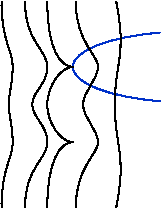
\includegraphics[height=2in]{main/Fig13-1}}
\caption{Cartier divisor on a smooth total space of a family of curves
that degenerates to a cuspidal curve; in this case the
limit of the associated family of invertible sheaves is invertible.}
\label{Fig13.1}
\end{figure}

Fortunately the ideal sheaves on cuspidal curves have a simple local
\index{ideal sheaf!on cuspidal curve}%
structure. The reason lies in the relation of the local ring $R_{0}$
of a cusp to its integral closure.

\begin{definition}
The \emph{conductor} of an integral domain $R_{0}$ is the annihilator
\index{conductor}%
of the $R_{0}$-module
$R/R_{0}$, where $R$ is the integral closure of $R_{0}$.
\unif
\end{definition}

It follows at once from the definition that the conductor of $R_{0}$
is also an ideal of $R$, and that it is the largest ideal of $R_{0}$
that is also
an ideal of $R$. The following result is a restatement of Example 2
after Proposition~\ref{Leray}:

\begin{proposition}\label{conductor of node and cusp}
If $R_{0}$ is the local ring of an ordinary cusp singularity of a curve,
then  $R/R_{0} \cong k$, the residue field of $R$, and thus the conductor
of $R_{0}$ is the
maximal ideal $\gm_{0}$ of $R_{0}$. \qed
\unif
\end{proposition}

\begin{proof} These properties can be verified after completing at the
maximal ideal of $R_{0}$.
To say
that $R_0$ has an ordinary cusp singularity means that the completion of
$R_0 \subset R$ is $k\[x^2,x^3\]\subset k\[x\]$, and the quotient is
$kx \cong k$.
\end{proof}


\begin{theorem}\label{torsion free at node}
Let $p$ be an ordinary cusp of a curve $C_0$ with normalization $\pi:
C \to C_0$. Let $R_0 = \sO_{C_0,p}$ be the local ring of the cusp,
with maximal ideal $\gm_0 = \sI_{p}R_{0}$,
and let $R_{0}\ruto {\pi^{*}} R$ be its normalization.  If $I_{0}\neq 0$
is an ideal of $R_{0}$ then
either $I_{0}\cong R_{0}$ or $I_{0}\cong \gm_0$.

 In the latter case, $I_{0} \cong Ra$, and if $R_{0}/I_{0}$ has length
 $v$ then $R/RI_{0} = R/I_{0}$ has length $v+1$.
 Moreover,
there is a split exact sequence
$$
0\to R/\gm_0 R \to R \otimes I_{0}  \to R I_{0} \to 0
$$
with $RI_{0}  \cong R$.
\unif
\end{theorem}

Interpreting Theorem~\ref{torsion free at node} in the context of an
ideal sheaf on a cuspidal curve
we get:

\begin{corollary}
Let $p\in C_{0}$ be an ordinary cusp in a reduced irreducible curve and
let $\pi:C \to C_{0}$ be
the partial normalization of $C_{0}$ at $p$, so that $p_a(C) = p_a(C_{0})-1$.
\index{partial normalization}%
Let $q\in C$ be the point lying over $p\in C_{0}$.

If $\sF_0$ is locally
isomorphic to a nonzero ideal sheaf on $C_{0}$
and $\sF_0$ is not locally free at $p$, then there is
a unique locally free sheaf $\sF$ on $C$ and a short exact sequence
$$
0\to \sO_{\pi^{-1}(p)} \to \pi^{*} \sF_{0} \to \sF \to 0.
$$
Thus $\chi(\sF) = \chi(\sF_{0}) -2$, so
$$
\deg@ \sF = \chi(\sF) - \chi(\widetilde \sO_{C}) =
\deg@\sF_{0}-1.
$$
Moreover, the map $H^{0}(\sF_{0}) \ruto {\pi^{*}} H^{0}(\sF(-q))$ is
a monomorphism.
\qed
\end{corollary}

\begin{proof}[Proof of Theorem~\ref{torsion free at node}]
The endomorphism ring of $I_0$ is commutative, it contains $R_0$,  and
\index{endomorphism ring}%
(since it stabilizes the finitely
generated module) it is integral over $R_0$. Thus
\index{integral!endomorphism ring}%
$$
R_0 \subset \End I_0 \subset R.
$$
Since
$R/R_0 \cong k$, the ring $\End I_0$ is equal to either
$R_0$ or $R$.

First, suppose
$\End I_{0}=R$, which is a discrete valuation ring. Every ideal of $R$
is principal, so we may write $I_{0} = Ra$.
 Since $\gm_0$ is also an ideal of $R$, it is isomorphic to $R$
as an $R$-module, and since $R_0\subset R$,
$I \cong \gm_0$ as $R_0$-modules. 
After completing we have
$\widehat R_{0} \cong \CC\[t^{2}, t^{3}, \dots\]$ and it is evident
that if $a$ has valuation $d$ in $R$ then the length of $R_{0}/(aR)$
is $d-1$, proving the claims in this case.

On the other hand, suppose
$\End I=R_0$
 and consider the inclusions
$$
\gm_0 I \subset I \subset R I.
$$
The left- and right-hand modules both have endomorphism ring $R$,
so both containments must be strict. Since $R/\gm_0$ has length 2,
we see that $I/\gm_0 I$ is principal. By 
\blue{Nakayama's lemma}
\index{Nakayama's lemma}%
$I\cong R_0$.
\end{proof}

Returning once again to the family $\cC \to \Delta$ at the beginning
of Section~\ref{Picard family}, assume that for general $t$ the scheme
$W^{r}_{d}(C_t)\neq \emptyset$. After replacing $\Delta$ with a
ramified covering we may assume that
$\sW^{r}_{d}(\sC/\Delta) \to \Delta$ has a section, that is, an
invertible sheaf $\sL$ on $\sC$ such that the restriction of $\sL$ to
each fiber $C_{t}$ with $t\neq 0$ has at least $r+1$ sections, so the
$g$-cuspidal curve $C_0$ that is the limit of this family has a
torsion-free sheaf $\cL_0$ of degree $d$. By the semicontinuity of
\index{semicontinuity!of cohomology}%
cohomology, $\sL_{0}$ also has at least $r+1$ sections.

At each cusp $r_i$ of $C_0$, $\cL_0$ is either locally free or
isomorphic to the maximal ideal of the cuspidal curve. Thus, if we
denote by $p_1,\dots, p_k$ the cusps of $C_0$ at which $\cL_0$ is
isomorphic to the maximal ideal, and let $C'_{0}$ be the partial
normalization of $C_0$ at those cusps, then $C'_{0}$ is a curve of
arithmetic genus $g-k$ having $g-k$ cusps, and the pullback of $\cL_0$
to $C'_{0}$ has at least $r$ sections with basepoints at the points
lying over $p_1,\dots,p_k$;  this is a $g^r_{d-k}$ on the
$(g-k)$-cuspidal curve~$D_0$.

\section{Putting it all together}
\label{nonexistence}

\subsection*{Nonexistence}

We can now prove that if $\rho(g,r,d) < 0$  then $W^{r}_{d}(C) =
\emptyset$ for curves in an open dense subset of $M_{g}$\emdash that is,
a general curve of genus $g$ does not possess a $g^r_d$.
Here we use Theorem~\ref{osculating intersection} from the last chapter,
which implies exactly this statement for invertible sheaves on an
arbitrary $g$-cuspidal curve $C_0$. If it were the case that a general
curve 
had
a $g^r_d$ with $\rho(g,r,d) < 0$, then by the results
of Section~\ref{Picard family}, there would be
 an invertible sheaf of degree $d$ with $\geq r+1$ sections on a
 $(g-k)$-cuspidal curve  $ C'_0$ for some $k \geq 0$. But since
$$
\rho(g-k, r, d-k) = \rho(g,r,d) - k < 0
,
$$
this is impossible by Theorem~\ref{osculating intersection}.

\subsection*{Existence}

Once more we let $\cC \to \Delta$ be a family of smooth
curves specializing to a $g$-cuspidal curve $C_0$. We can 
combine
Corollary~\ref{intersection with sigma nonzero} with
Theorem~\ref{osculating intersection} to 
show
that the variety $W^r_d(C_0)$
is nonempty of dimension $\rho(g,r,d)$. Since the codimension of
$\cW^r_d(\cC/\Delta) \subset \pic_d(\cC/\Delta)$ is at most $(r+1)(g-d+r)$
locally everywhere, we may conclude, by the semi-continuity of fiber dimension, that likewise for general $t$
the variety $W^r_d(C_t)$ is nonempty of dimension exactly $\rho(g,r,d)$.

\section{Brill--Noether with inflection}

The approach we've taken here to the proof of Brill--Noether is
\index{linear series on $\PP^1$!inflections}%
\index{inflectionary behavior}%
\index{Brill--Noether theorem!with inflection}%
well-suited to analyzing the inflectionary behavior of linear series on a
general curve; indeed, a small modification of the argument above allows
us to prove a stronger form of the Brill--Noether statement, concerning
the existence of $g^r_d$s on a general curve $C$ that are required to
 have inflection points of given weights.

\begin{definition}
Let $C$ be a smooth curve of genus $g$ and $p_1,\dots,p_n \in C$ distinct
points of $C$. If $\cD = (L,V)$ is a linear system on $C$ of degree $d$
and dimension $r$, we define the \emph{adjusted Brill--Noether number}
\index{Brill--Noether number!adjusted}%
of $\cD$ relative to the points $p_k$ to be
$$
\rho(\cD; p_1,\dots,p_k) \colonequals  g - (r+1)(g-d+r) - \sum_{k=1}^n
w(\cD,p_k).
$$
\end{definition}

In these terms, we can prove 
a
generalization of the
``nonexistence'' half of Brill--Noether:

\begin{theorem}\label{Brill--Noether with inflection}
Let $(C;p_1,\dots,p_n)$ be a general $n$-pointed curve of genus $g$
(that is, let $C$ be a general curve and $p_1,\dots,p_n \in C$ general
points). If $\cD$ is any linear system on $C$, then
$$
\rho(\cD; p_1,\dots,p_n) \geq 0.
$$
\end{theorem}

\begin{proof}
To start, let $\cC \to \Delta$ be a family of curves as in the proof of
Lemma~\ref{specialization to cuspidal curve}.
As in the argument
at the start of Section~\ref{nonexistence},
possibly
after pulling back the family along a ramified map $\Delta \to \Delta$,
we can choose sections $\sigma_1, \dots, \sigma_n : \Delta \to \cC$
of $\cC \to \Delta$ such that the $\sigma_k(0)$ are distinct smooth
points of $C_0$.
If the general curve $C_b$ in our family admits a $g^r_d$ $\cD$ with
$$
\rho(\cD;\sigma_1(b),\dots,\sigma_n(b)) < 0
$$
then, possibly after pulling the family back along a ramified map $\Delta
\to \Delta$, we can choose a family $\{\cD_b\}$ of such linear series
on the fibers $C_b$ for $b \neq 0$ and, taking limits, we arrive at a
$g^r_d$ $\cD_0$ on $\PP^1$ with
$$
w(\cD_0, q_i) \geq r
$$
for each of the $g$ points $q_i \in \PP^1$ lying over the cusps of $C_0$,
and in addition
$$
w(\cD_0, r_k) \geq w(\cD_b,\sigma_k(b))
$$
where $r_k \in \PP^1$ is the point in $\PP^1$ lying over $\sigma_k(0)
\in C_0$. Adding up, we have
\begin{align*}
\sum_{i=1}^g w(\cD_0, q_i) + \sum_{k=1}^n w(\cD_0, r_i) &\geq rg +
\sum_{k=1}^n w(\cD_b,\sigma_k(b)) \\
&> rg + g - (r+1)(g-d+r) = (r+1)(d-r)
,
\end{align*}
since we assumed that
$$
\rho(\cD_b;\sigma_1(b),\dots,\sigma_n(b)) = g - (r+1)(g-d+r) -
\sum_{k=1}^n w(\cD_b,\sigma_k(b)) < 0.
$$
But as before the Pl\"ucker formula for $\PP^1$ tells us that
$$
\sum_{p \in \PP^1} w(\cD_0, p) = (r+1)(d-r),
$$
a contradiction.
\end{proof}

This extension of the ``nonexistence'' part of
the Brill--Noether theorem
raises
the question of a converse: if $(C;p_1,\dots,p_n)$ is a general
$n$-pointed curve of genus $g$, and we specify ramification sequences
$\alpha^1, \dots, \alpha^n` `$, can we say that there exists a $g^r_d$
$\cD$ on $C$ with $\alpha_i(\cD, p_k) \geq \alpha^k_i$ for
$k=1,\dots,n$ and $i = 0, \dots, r$? If the product of the
corresponding
\blue{Schubert classes}
\index{Schubert classes}%
in $G(d-r, d+1)$ is nonzero, then we
can indeed deduce the existence of such a linear series; and if the
product is 0, we can deduce that no such linear series exists.

Here is one way to state what we know without getting lost in a thicket
of Schubert calculus:

\begin{theorem}\label{BN with inflection and dimension}
Let $C$ be a smooth curve of genus $g$ and $p_1,\dots,p_n \in C$ distinct
points; for $k = 1,\dots,n$ let $\alpha^k = (\alpha^k_0,\dots\alpha^k_r)$
be a nondecreasing sequence of nonnegative integers, and let
$$
G^r_d(p_1,\dots,p_n; \alpha^1,\dots,\alpha^n) = \{\cD \in G^r_d(C)
\mid \alpha_i(\cD, p_k) \geq \alpha^k_i \}.
$$
If $@(C, p_1,\dots,p_n)$ is a general $n$-pointed curve, 
then either
$$
G^r_d(p_1,\dots,p_n; \alpha^1,\dots,\alpha^n) 
$$
is empty, or it has dimension
$$
%\dim G^r_d(p_1,\dots,p_n; \alpha^1,\dots,\alpha^n) = 
\rho(g,r,d) -
\sum_{k+1}^n \sum_{i=0}^r \alpha^k_i.
$$
\end{theorem}

Finally, from the codimensions of the Schubert varieties  we can deduce
the ramification behavior of general
linear series:

\begin{theorem}
If $\cD$ is a general $g^r_d$ on a general curve, then $\cD$ has only
\index{ramification!simple}
\index{Weierstrass point)}%
simple ramification; that is,
$$
w(\cD, p) \leq 1 \quad \text{for all } p \in C.
$$
\end{theorem}

Applying this in case $d=2g-2$ and $r = g-1$, we arrive at the
statement made
after Corollary~\ref{Weierstrass points}:
that a general
curve $C$ of genus $g$ has only Weierstrass points of weight 1.

\section{Exercises}

\begin{exercise}
  By Theorem~\ref{BN with inflection and dimension}, there is a $g^1_4$
  on a general curve $C$ of 
\blue{genus 3} 
ramified at any 2 general points $p,
\index{g@$g^1_4$}%
\index{genus 3}%
  q \in C$. Construct it.

  Hint: Using the canonical embedding to realize $C$ as a 
\blue{plane quartic}
\index{plane quartic}%
  and project from the point of intersection of the tangent lines at $p$
  and $q$.
\end{exercise}

The 
next 
three exercises give the results necessary to prove
Theorem~\ref{BN-basic} using degeneration to
\blue{nodal curves}
\index{nodal curve}%
rather than to cuspidal curves.

\begin{exercise}[construction of nodal curves]
\label{independent secants}
\label{Constructing nodal curves} 
Let $C$ be a smooth curve,
and let
 $\{(p_{i}, q_{i}) \mid i = 1\dots h\}$ be $2h$ distinct points of $C$.

Show that if $C$ is embedded in $\PP^{r}$ by a complete linear series
of sufficiently high degree, then the
projection of $C$ from a general $(r-4)$-plane $\Lambda$ that meets each
secant $\overline{p_{i} q_{i}}$
maps $C$ to a curve with $h$ ordinary nodes in $\PP^{3}$.

Hint: Use dimension counts to show that:
\begin{enumerate}
\item $\Lambda$ does not contain any tangent line to $C$.
\item $\Lambda$ does not meet any secant line to $C$ other than the
lines  $\overline{p_{i} q_{i}}$.
\item $\Lambda$ does not meet the 3-plane $\overline{\TT_{p_i}C,
\TT_{q_i}C}$ in a line.
\end{enumerate}
 \end{exercise}

\begin{exercise}\label{BN via nodal curves}\label{secant general position}
Suppose that $C\subset \PP^{d}$ is the rational normal curve of degree
$d$, and $\{L_{i} = \overline{p_{i}q_{i}}\}$
is a collection of secants of $C$. Show that if the points $p_{i},
q_{i}\in C$ are chosen sufficiently generally,
then any collection of Schubert cycles $\Sigma_{a_{i}}(L_{i})$ meet
dimensionally transversely.

Hint: Let the $p_{i}, q_{i}$ approach each other, reducing to the case
of tangent lines. Then use
Theorem~\ref{osculating intersection}. For a direct proof see \cite[Lemma,
p.~259]{Griffiths-Harris-BN}.
\end{exercise}

\begin{exercise}\label{linear series on a nodal curve}
Imitate the proof of Proposition~\ref{torsion free on cuspidal} to
show that if $R_{0}$ is the local ring of a node\emdash that is, the
completion $\widehat R$ is isomorphic to $\CC[x,y]/(xy)$\emdash then
every nonzero ideal of $R$ is isomorphic
either to $R$ or to the maximal ideal of $R$. Deduce that if $C\to C_{0}$
is the
partial normalization of a single node on a reduced irreducible projective
curve, then there is an exact sequence
$$0\to \CC^{*} \to \pic_{0}(C_{0}) \to \pic_{0}(C) \to 0.$$

Hint:
Let $C_{0}$ be a curve with a node $p$, and $C \ruto {\,\nu} C_{0}$
\index{partial normalization}%
its 
\blue{partial normalization}
at $p$. Denote by $q,r \in \widetilde C$
the points lying over $p$. If $\cL$ is an invertible sheaf on $C$, and
$\cM \colonequals  \nu^*(\cL)$ the pullback of $\cL$ to $\widetilde C$,
then $\cM$ is an invertible sheaf on $\widetilde C$. Its fibers over $q$
and $r$ are both identified with the fiber $\cL_p$ of $\cL$ at $p$, and
hence with each other. Conversely, given an invertible sheaf $\cM$ on
$\widetilde C$ and an identification of the fibers $\cM_q$ and $\cM_r$,
we can form an invertible sheaf $\cL$ on $C$ by taking the subsheaf
of $\nu_*\cM$ whose sections agree at $q$ and $r$, in terms of the
identification.
\end{exercise}

%footer for separate chapter files

\ifx\whole\undefined
%\makeatletter\def\@biblabel#1{#1]}\makeatother
\makeatletter \def\@biblabel#1{\ignorespaces} \makeatother
\bibliographystyle{msribib}
\bibliography{slag}

%%%% EXPLANATIONS:

% f and n
% some authors have all works collected at the end

\begingroup
%\catcode`\^\active
%if ^ is followed by 
% 1:  print f, gobble the following ^ and the next character
% 0:  print n, gobble the following ^
% any other letter: normal subscript
%\makeatletter
%\def^#1{\ifx1#1f\expandafter\@gobbletwo\else
%        \ifx0#1n\expandafter\expandafter\expandafter\@gobble
%        \else\sp{#1}\fi\fi}
%\makeatother
\let\moreadhoc\relax
\def\indexintro{%An author's cited works appear at the end of the
%author's entry; for conventions
%see the List of Citations on page~\pageref{loc}.  
%\smallbreak\noindent
%The letter `f' after a page number indicates a figure, `n' a footnote.
}
\printindex[gen]
\endgroup % end of \catcode
%requires makeindex
\end{document}
\else
\fi
